%%%%%%%%%%%%%%%%%%%%%%%%%%%%%%%%%%%%%%%%%%%%%%%%%%%%%%%%%%%%%%%%%%%%%%
% How to use writeLaTeX: 
%
% You edit the source code here on the left, and the preview on the
% right shows you the result within a few seconds.
%
% Bookmark this page and share the URL with your co-authors. They can
% edit at the same time!
%
% You can upload figures, bibliographies, custom classes and
% styles using the files menu.
%
%%%%%%%%%%%%%%%%%%%%%%%%%%%%%%%%%%%%%%%%%%%%%%%%%%%%%%%%%%%%%%%%%%%%%%

\documentclass[12pt]{article}

\usepackage{sbc-template}

\usepackage{graphicx,url}

%\usepackage[brazil]{babel}   
\usepackage[utf8]{inputenc}  

\usepackage{tikz}

\usetikzlibrary{arrows.meta, positioning, backgrounds}
     
\sloppy

\title{Exercício 1 do Grau B de Sistemas Distribuídos}

\author{Christian Aguiar Plentz\inst{1}, João Roberto Lemos Fidellis\inst{2} 
, Julian Rafael de Souza\inst{3}}


\address{Ciência da Computação -- Universidade do Vale do Rio dos Sinos (UNISINOS)\\
  Caixa Postal 275 -- 93022-750 -- São Leopoldo -- RS -- Brazil
  \email{\{plentzchristian,JRFIDELLIS,julian93\}@edu.unisinos.br}
}


\begin{document} 

\maketitle

\section{Relógios Lógicos de Lamport}

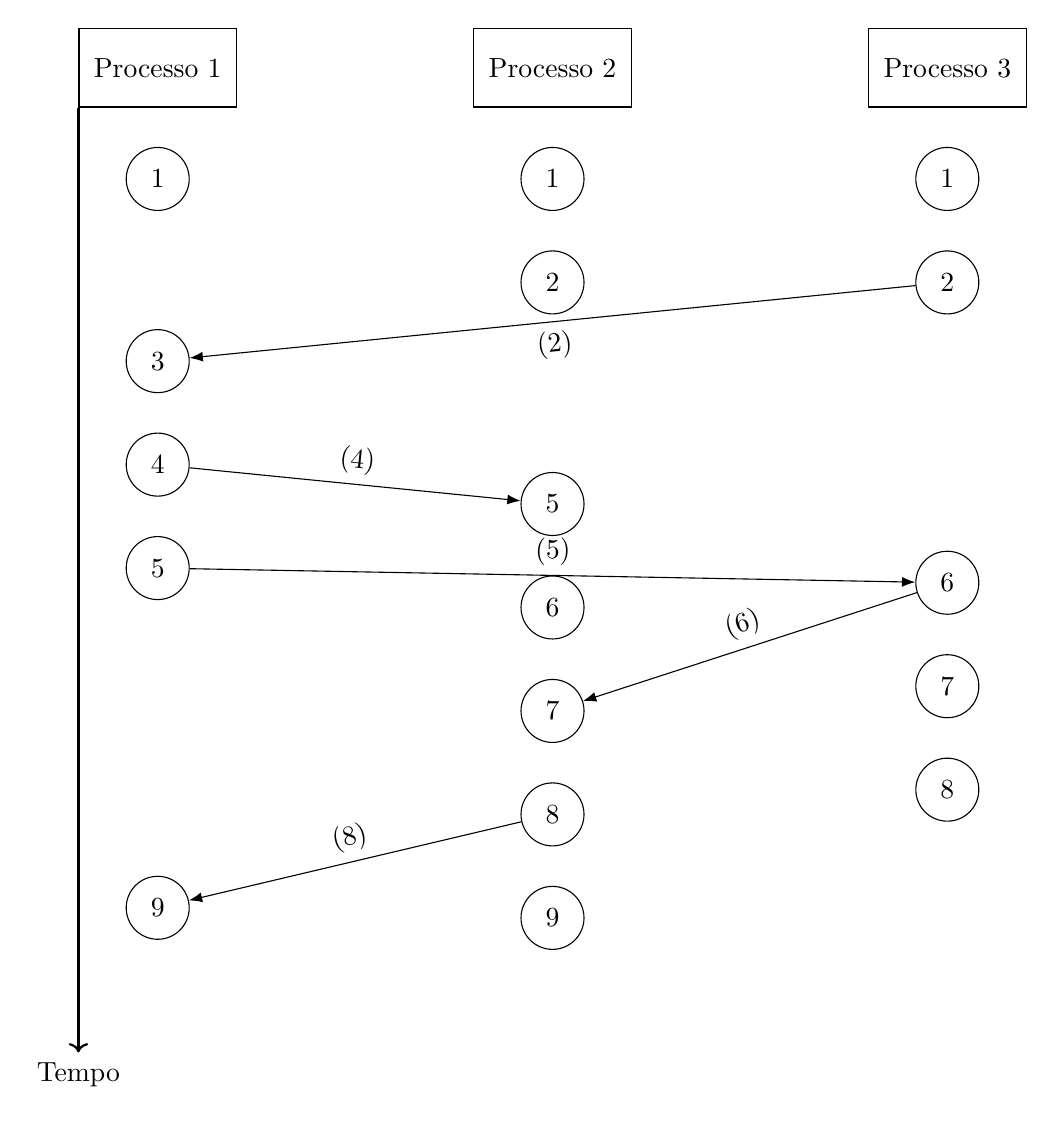
\begin{tikzpicture}[
    node distance=1cm,
    event/.style={circle, draw, minimum size=0.8cm},
    process/.style={rectangle, draw, minimum width=2cm, minimum height=1cm}
]


% Processes
\node[process] (p1) {Processo 1};
\node[process, right=3cm of p1] (p2) {Processo 2};
\node[process, right=3cm of p2] (p3) {Processo 3};


% Process 1 events
\node[event, below=0.5cm of p1] (a1) {1};
\node[event, below=1.5cm of a1] (a2) {3};
\node[event, below=0.5cm of a2] (a3) {4};
\node[event, below=0.5cm of a3] (a4) {5};
\node[event, below=3.5cm of a4] (a5) {9};

% Process 2 events
\node[event, below=0.5cm of p2] (b1) {1};
\node[event, below=0.5cm of b1] (b2) {2};
\node[event, below=2cm of b2] (b3) {5};
\node[event, below=0.5cm of b3] (b4) {6};
\node[event, below=0.5cm of b4] (b5) {7};
\node[event, below=0.5cm of b5] (b6) {8};
\node[event, below=0.5cm of b6] (b7) {9};

% Process 3 events
\node[event, below=0.5cm of p3] (c1) {1};
\node[event, below=0.5cm of c1] (c2) {2};
\node[event, below=3cm of c2] (c3) {6};
\node[event, below=0.5cm of c3] (c4) {7};
\node[event, below=0.5cm of c4] (c5) {8};

% Message arrows
\draw[-Latex] (c2) -- node[below, sloped] {(2)} (a2);
\draw[-Latex] (a3) -- node[above, sloped] {(4)} (b3);
\draw[-Latex] (a4) -- node[above, sloped] {(5)} (c3);
\draw[-Latex] (c3) -- node[above, sloped] {(6)} (b5);
\draw[-Latex] (b6) -- node[above, sloped] {(8)} (a5);

% Time arrows
\draw[->, thick] (p1.south west) -- ++(0,-12) node[below] {Tempo};

\end{tikzpicture}

\section{Vetor de Timestamps}

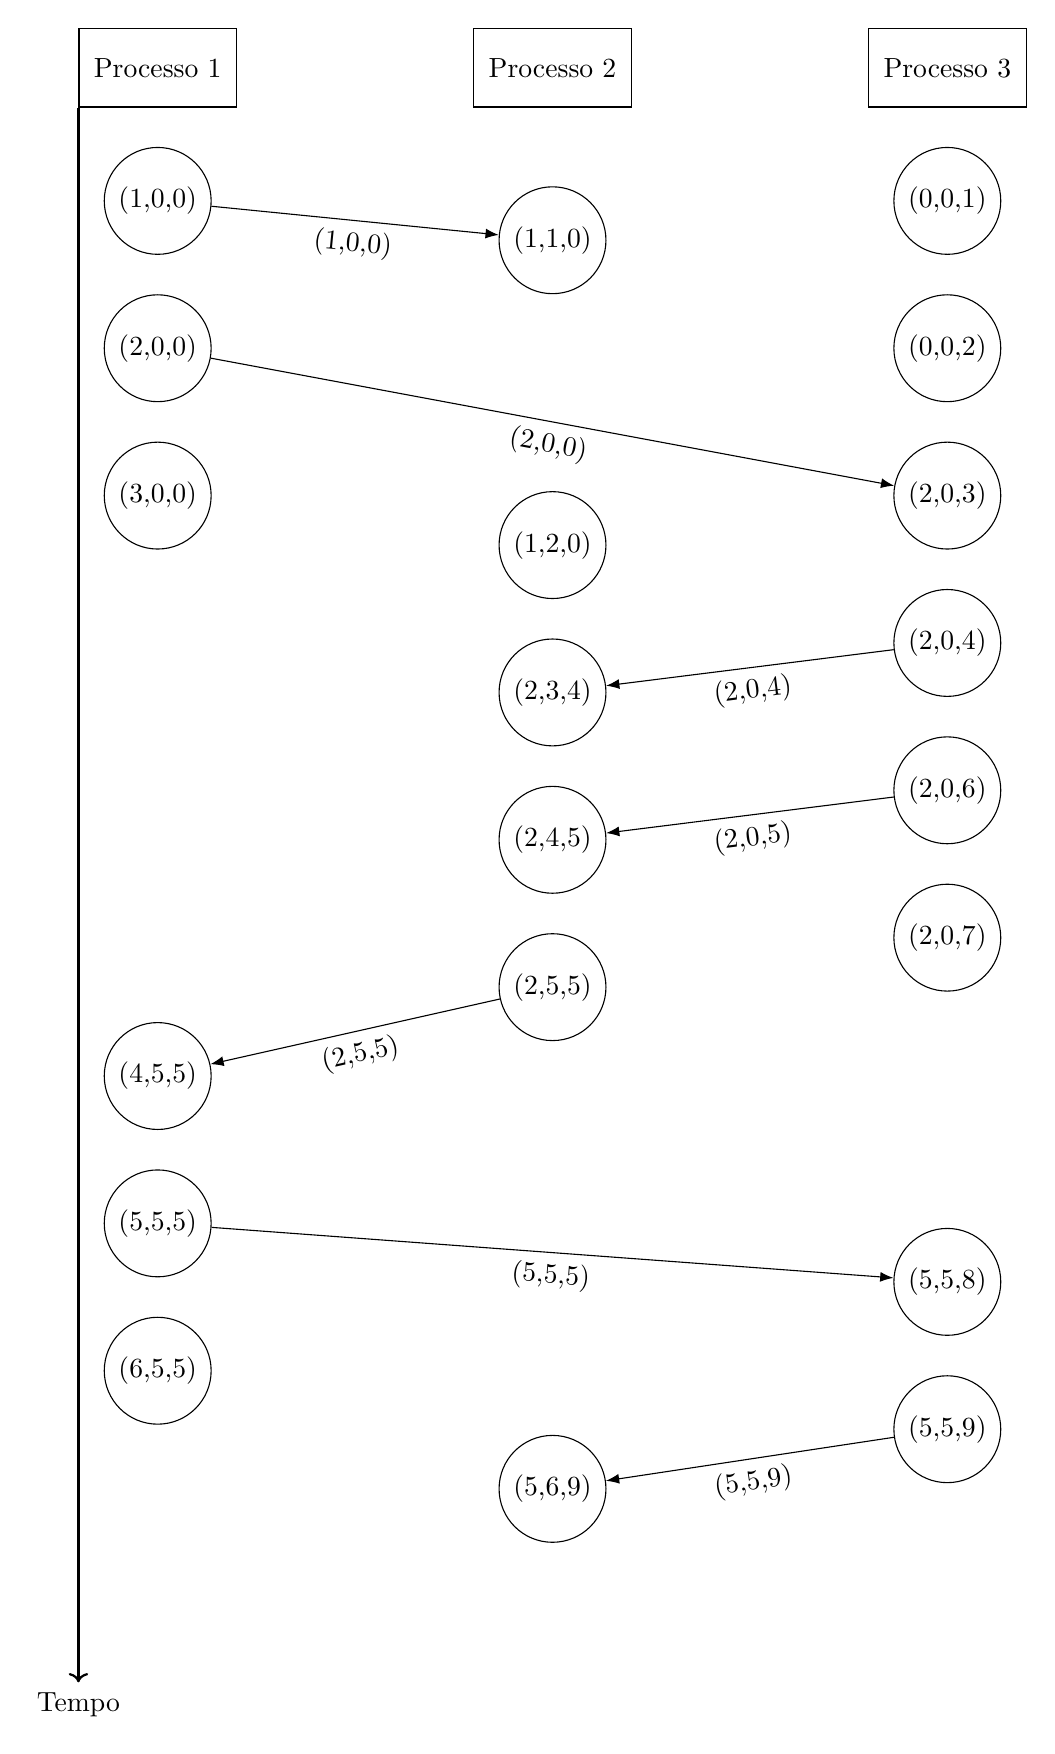
\begin{tikzpicture}[
    node distance=1cm,
    event/.style={circle, draw, minimum size=0.8cm},
    process/.style={rectangle, draw, minimum width=2cm, minimum height=1cm}
]


% Processes
\node[process] (p1) {Processo 1};
\node[process, right=3cm of p1] (p2) {Processo 2};
\node[process, right=3cm of p2] (p3) {Processo 3};


% Process 1 events
\node[event, below=0.5cm of p1] (a1) {(1,0,0)};
\node[event, below=0.5cm of a1] (a2) {(2,0,0)};
\node[event, below=0.5cm of a2] (a3) {(3,0,0)};
\node[event, below=6cm of a3] (a4) {(4,5,5)};
\node[event, below=0.5cm of a4] (a5) {(5,5,5)};
\node[event, below=0.5cm of a5] (a6) {(6,5,5)};

% Process 2 events
\node[event, below=1cm of p2] (b1) {(1,1,0)};
\node[event, below=2.5cm of b1] (b2) {(1,2,0)};
\node[event, below=0.5cm of b2] (b3) {(2,3,4)};
\node[event, below=0.5cm of b3] (b4) {(2,4,5)};
\node[event, below=0.5cm of b4] (b5) {(2,5,5)};
\node[event, below=5cm of b5] (b6) {(5,6,9)};

% Process 3 events
\node[event, below=0.5cm of p3] (c1) {(0,0,1)};
\node[event, below=0.5cm of c1] (c2) {(0,0,2)};
\node[event, below=0.5cm of c2] (c3) {(2,0,3)};
\node[event, below=0.5cm of c3] (c4) {(2,0,4)};
\node[event, below=0.5cm of c4] (c5) {(2,0,6)};
\node[event, below=0.5cm of c5] (c6) {(2,0,7)};
\node[event, below=3cm of c6] (c7) {(5,5,8)};
\node[event, below=0.5cm of c7] (c8) {(5,5,9)};

% Message arrows
\draw[-Latex] (a1) -- node[below, sloped] {(1,0,0)} (b1);
\draw[-Latex] (a2) -- node[below, sloped] {(2,0,0)} (c3);
\draw[-Latex] (c4) -- node[below, sloped] {(2,0,4)} (b3);
\draw[-Latex] (c5) -- node[below, sloped] {(2,0,5)} (b4);
\draw[-Latex] (b5) -- node[below, sloped] {(2,5,5)} (a4);
\draw[-Latex] (a5) -- node[below, sloped] {(5,5,5)} (c7);
\draw[-Latex] (c8) -- node[below, sloped] {(5,5,9)} (b6);

% Time arrows
\draw[->, thick] (p1.south west) -- ++(0,-20) node[below] {Tempo};

\end{tikzpicture}


\end{document}


